\documentclass[main.tex]{subfiles} % Subfile-Class


% ============================================================================== %
%                            Subfile document                                    %
% ============================================================================== %

\begin{document}

% Template

\subsubsection{Antriebe und Dimensionierung}

Dieser Abschnitt befasst sich mit der Auswahl eines geeigneten Antriebs mit
Steuerung für den Roboter. Die Evaluation der Antriebe,
sieheAnhang~\ref{appendix:Antriebe}, hat ergeben, dass ein Schrittmotor der
FirmaDFRobot, siehe Abbildung~\ref{Schrittmotor_FIT0278}, eingesetzt wird.
Dieser ist in der Lage, den Roboter mit 1.7A auf bis zu $2\frac{m}{s}$ zu
beschleunigen.
\begin{figure}[H]
    \centering
    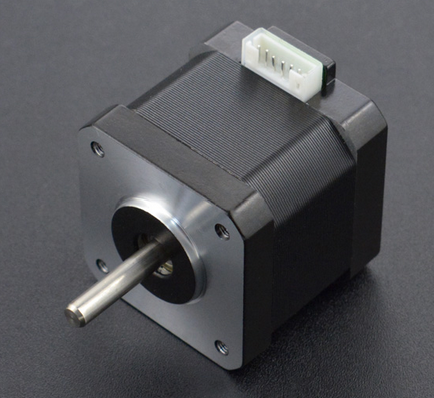
\includegraphics[width = 0.25 \linewidth]{fig_Antriebe_und_Dimensionierung/DFRobot_Stepper_FIT0278.png}
    \caption{Schrittmotor}~\label{Schrittmotor_FIT0278}
\end{figure}

\begin{figure}[H]
    \centering
    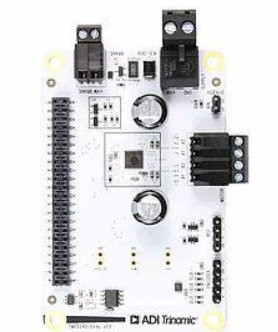
\includegraphics[width = 0.25 \linewidth]{fig_Antriebe_und_Dimensionierung/TMC_5240_EVAL.png}
    \caption{Evaluationboard TMC5240}~\label{Schrittmotorentreiber_EVAL}
\end{figure}

Die Ansteuerung dieser Motoren erfolgt über einen
vollintegriertenSchrittmotortreiber der Firma ADI-Trinamic. Um den
Entwicklungsaufwand geringzu halten, wird auf 2 Evaluation-Boards des
Treiber-IC's \textit{TMC-5240}zurückgegriffen, wie in
Abbildung~\ref{Schrittmotorentreiber_EVAL} gezeigt.Eines der Teammitglieder hat
bereits Erfahrung mit diesem speziellen Treiberund kann auf entsprechende
Treiber-Evaluation-Boards aus seinem beruflichenUmfeld zurückgreifen.

Abbildung~\ref{Ansteuerungstopologie_Schrittmotorentreiber} zeigt
schematisch,wie diese Treiber angesteuert werden.

\begin{figure}[H]
    \centering
    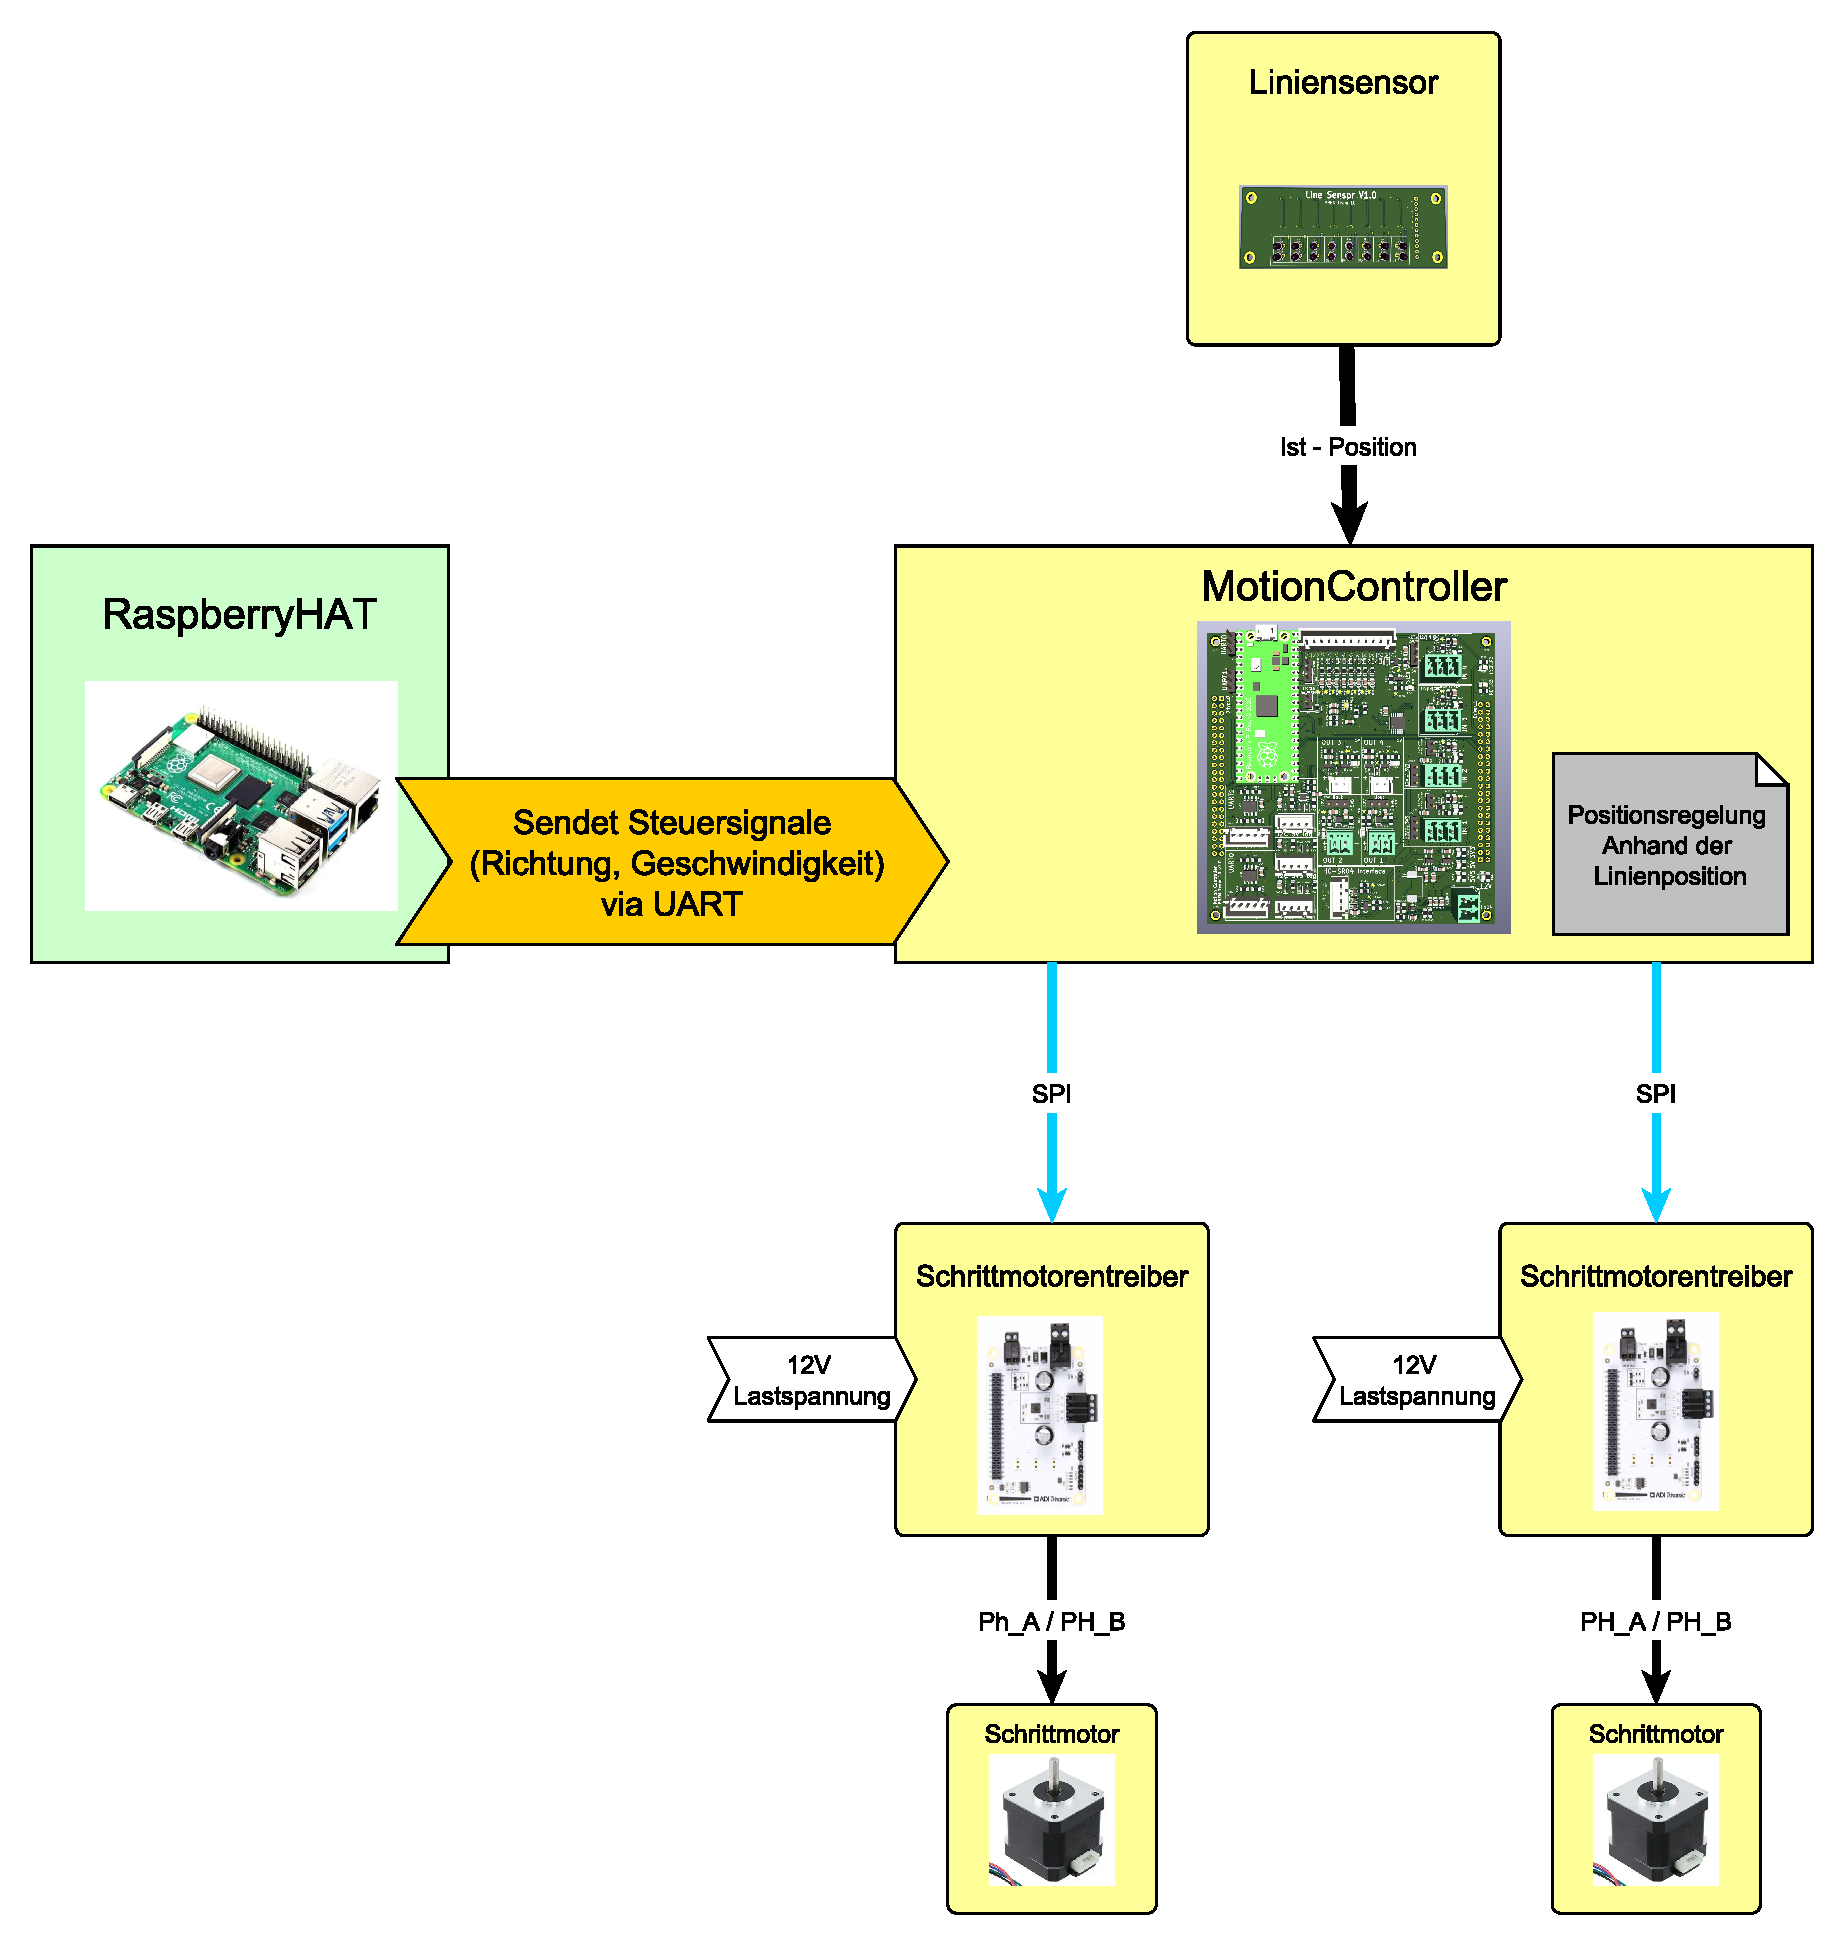
\includegraphics[width = 1\linewidth]{fig_Antriebe_und_Dimensionierung/Konzept_Motoransteuerung.pdf}
    \caption{Ansteuerungstopologie Schrittmotoren}~\label{Ansteuerungstopologie_Schrittmotorentreiber}
\end{figure}

Die Antriebsregelung ist auf einer separaten Leiterplatte realisiert. Als
Eingangssignal für diese Regelung dient nur der Liniensensor. Die Ansteuerung
der beiden Schrittmotortreiber erfolgt über den SPI-Bus des Mikrocontrollers.

An den Rädern sind zusätzlich Encoder vorgesehen, damit der Navigationsrechner
den zurückgelegten Weg verfolgen kann. Aus Gründen der Echtzeitfähigkeit bei
der Auswertung der Encoder werden diese auf der Antriebssteuerung und nicht auf
dem Navigationsrechner ausgewertet. Die Encoder stellen im aktuellen
Projektstand eine Fallback-Lösung dar. Im Folgemodul wird noch evaluiert, ob
die gefahrenen Schritte, die aus dem Motortreiber ausgelesen werden können,
ausreichen, um die gefahrene Strecke rekonstruieren zu können.

Signale, in welche Richtung das Fahrzeug bewegt werden soll, sowie Start- und
Stoppsignale erhält der Mikrocontroller vom Navigationsrechner über eine
UART-Schnittstelle. Ebenfalls über UART kann der Greifcontroller Signale an den
Antriebscontroller senden, die die Antriebe stoppen - das Fahrzeug drehen oder
weiterfahren lassen.

Abbildung~\ref{fig:Blockschaltbild_Motioncontroller} zeigt schematisch, welche
Funktionsgruppen auf der entsprechenden Platine enthalten sind.

\begin{figure}[H]
    \centering
    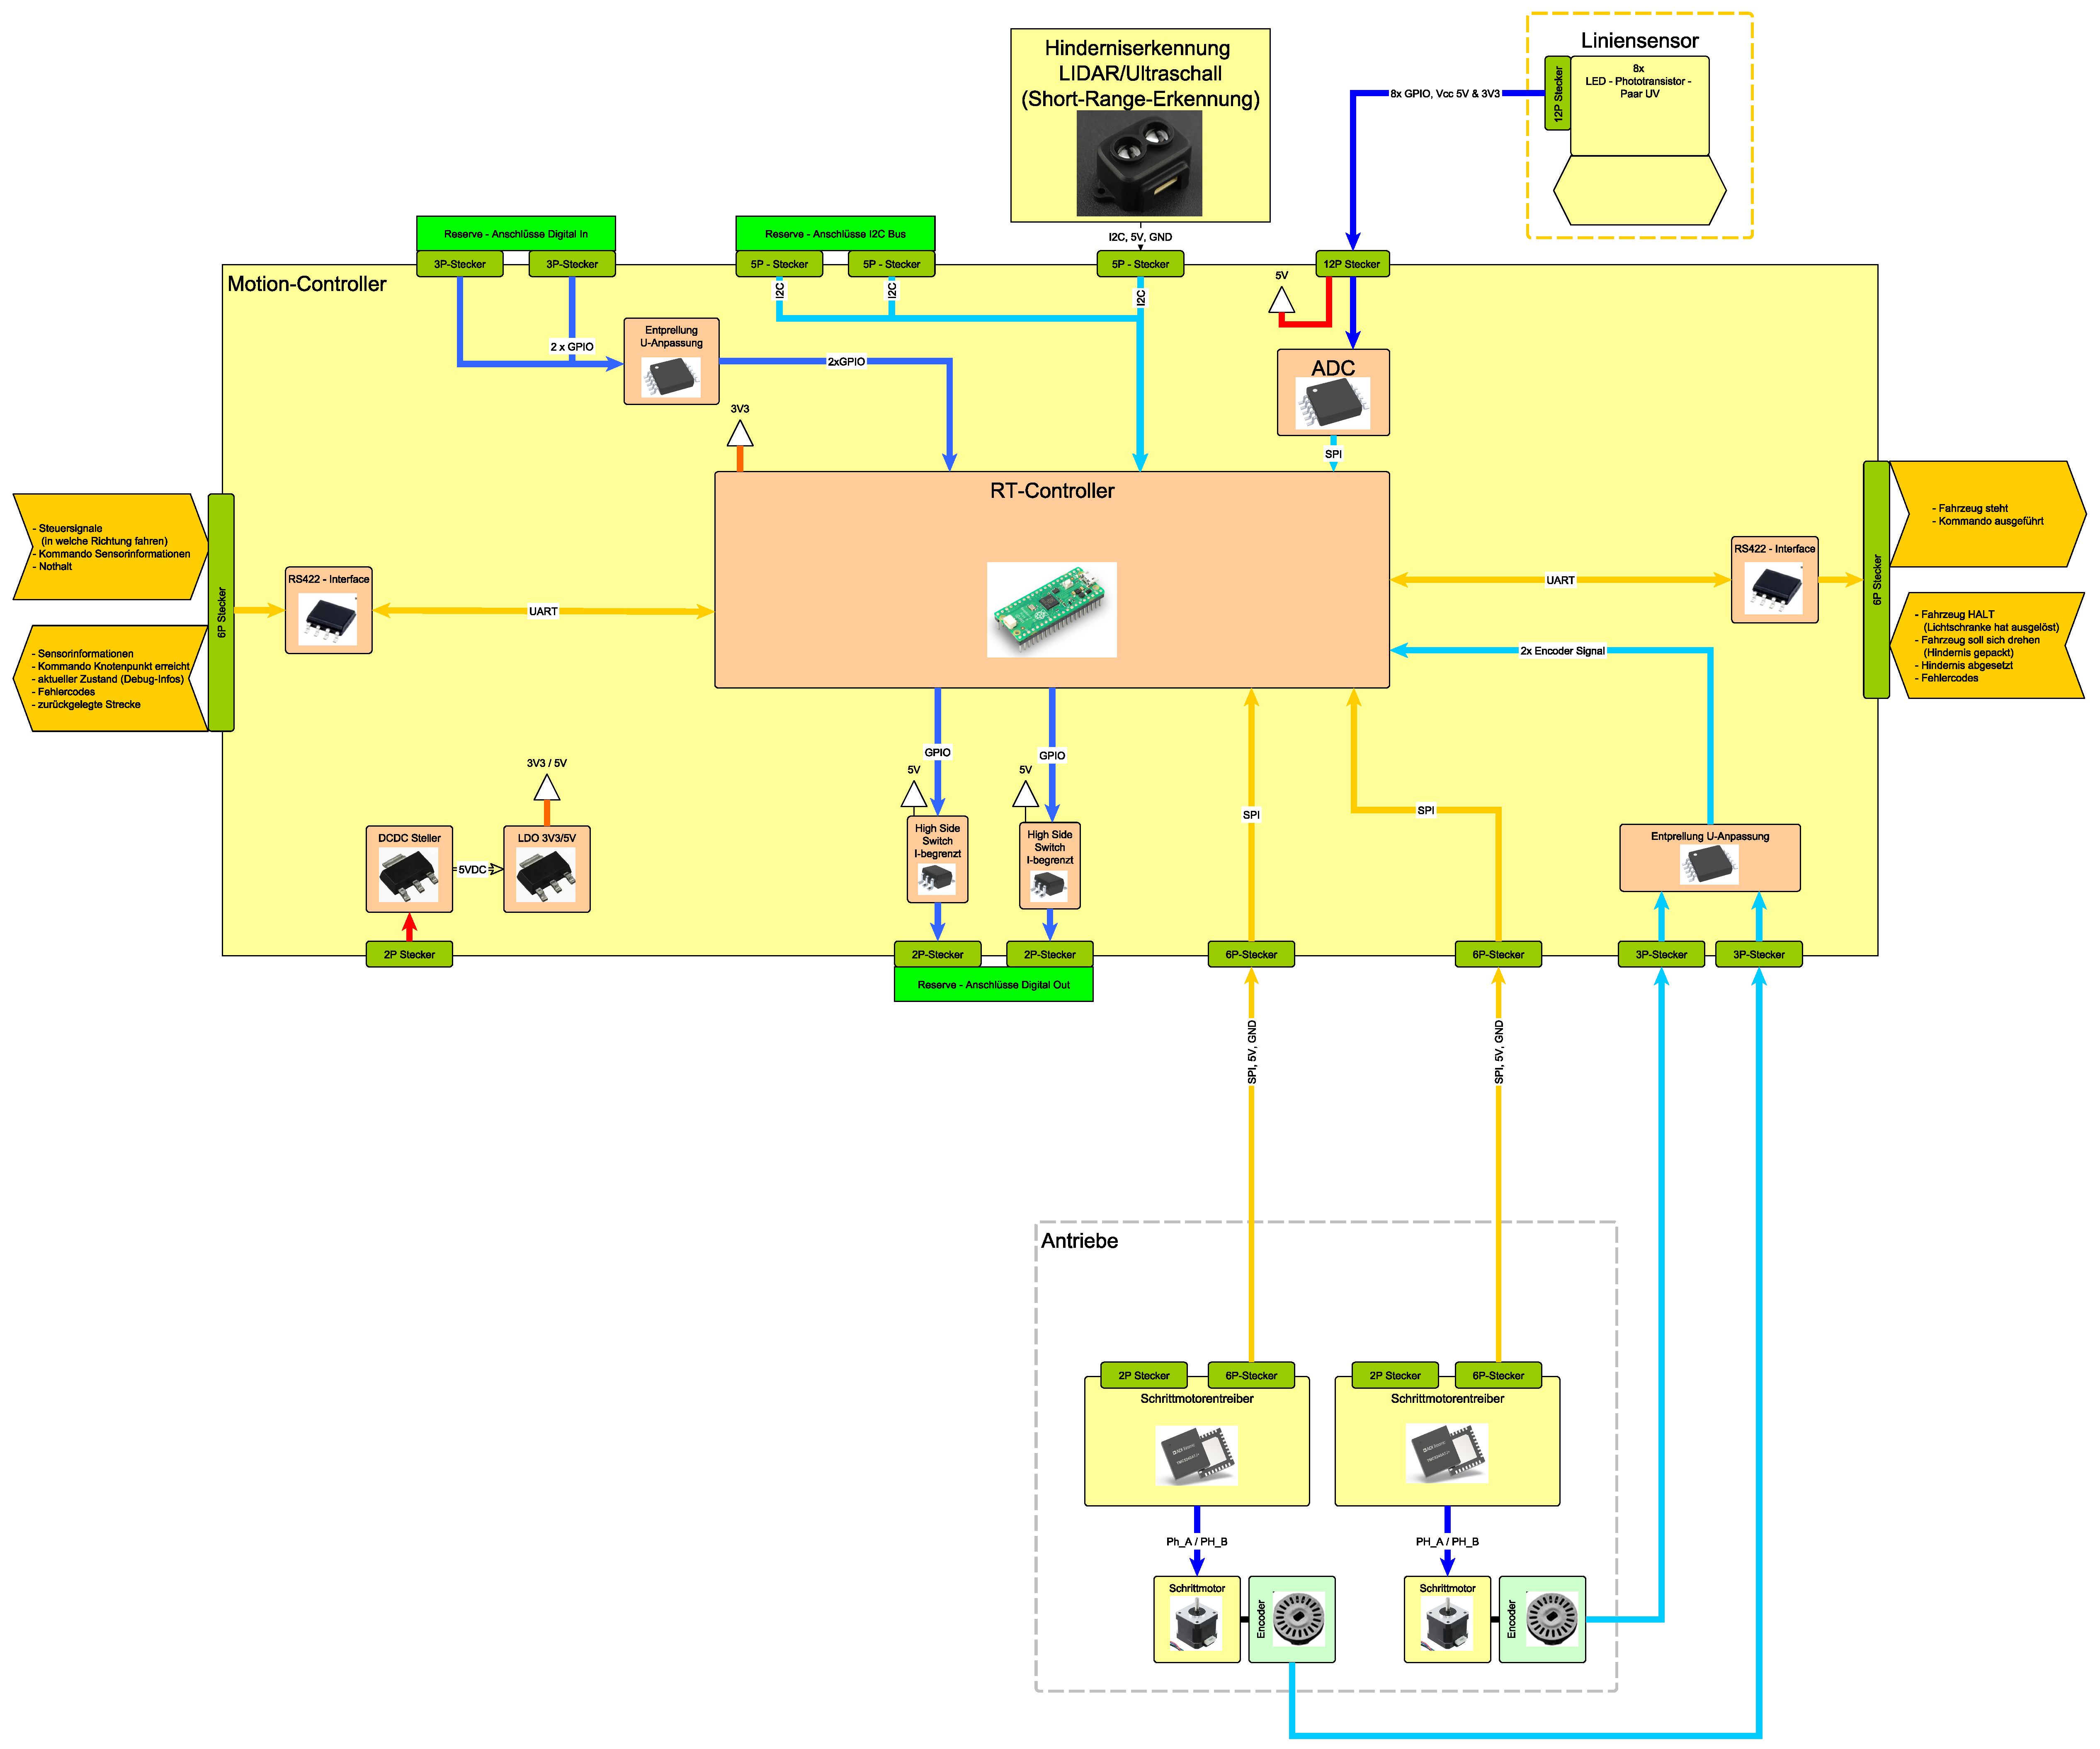
\includegraphics[width = 1\linewidth]{fig_Antriebe_und_Dimensionierung/MotionController_Blockschaltbild.pdf}
    \caption{Blockschaltbild Motion Controller}~\label{fig:Blockschaltbild_Motioncontroller}
\end{figure}

Der Motion Controller verfügt über digitale Ein- und Ausgänge mit schaltbaren
Spannungspegeln als Reserve, falls im Verlauf des Folgemoduls PREN2 Sensoren
angepasst oder zusätzliche Aktoren hinzugefügt werden
müssen.Abbildung~\ref{fig:MotionBoard_PCB} zeigt das Motion Controller PCB in
einer 3D-Ansicht. Es verfügt über 3 $I^2C$-Anschlüsse, ein spezielles
HC-SR04-Ultraschallsensor-Interface und die bereits erwähnten digitalen
Ein-/Ausgänge. Zusätzlich ist eine Schnittstelle für den Liniensensor
vorgesehen und ein Gyroskop zur Winkelerfassung integriert. Es wird wie eine
Brücke auf die beiden Evaluation Boards von Trinamic gesteckt, wofür sich die
breiten Steckerleisten an den Aussenkanten befinden.

\begin{figure}[H]
    \centering
    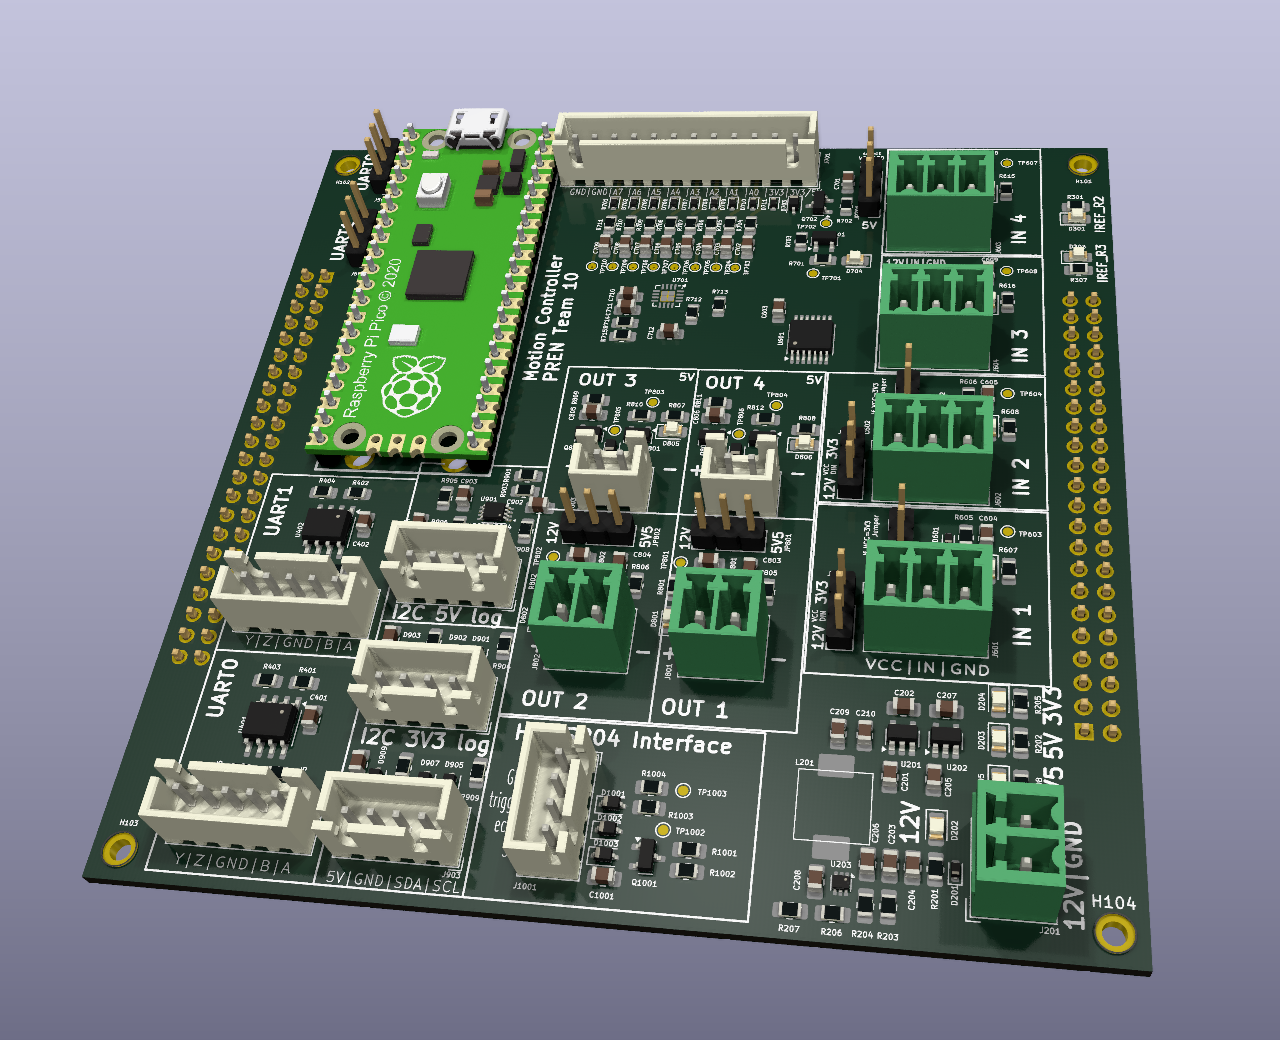
\includegraphics[width = 0.75\linewidth]{fig_Antriebe_und_Dimensionierung/MotionControllerPCB.jpg}
    \caption{3D-Ansicht Motion Controller}~\label{fig:MotionBoard_PCB}
\end{figure}

\end{document}

Nach dem derzeitigen Stand des Konzepts für PREN1 wäre dieser Controller in der
Lage, auch die Aufgabe des Greifers zu übernehmen. Es ist jedoch nicht ganz
klar, inwieweit der Greifer in seinem jetzigen Zustand implementiert werden
kann und ob noch weitere Ein-/Ausgänge benötigt werden. Daher ist für das
Folgemodul eine eigene Platine für die Greiferaufgabe vorgesehen.

\subsubsection*{Software}

Im Nachfolgemodul ist die Entwicklung der Firmware des MotionControllers in C++
auf Basis des FreeRTOS-Kernels geplant.

\begin{figure}[H]
    \centering
    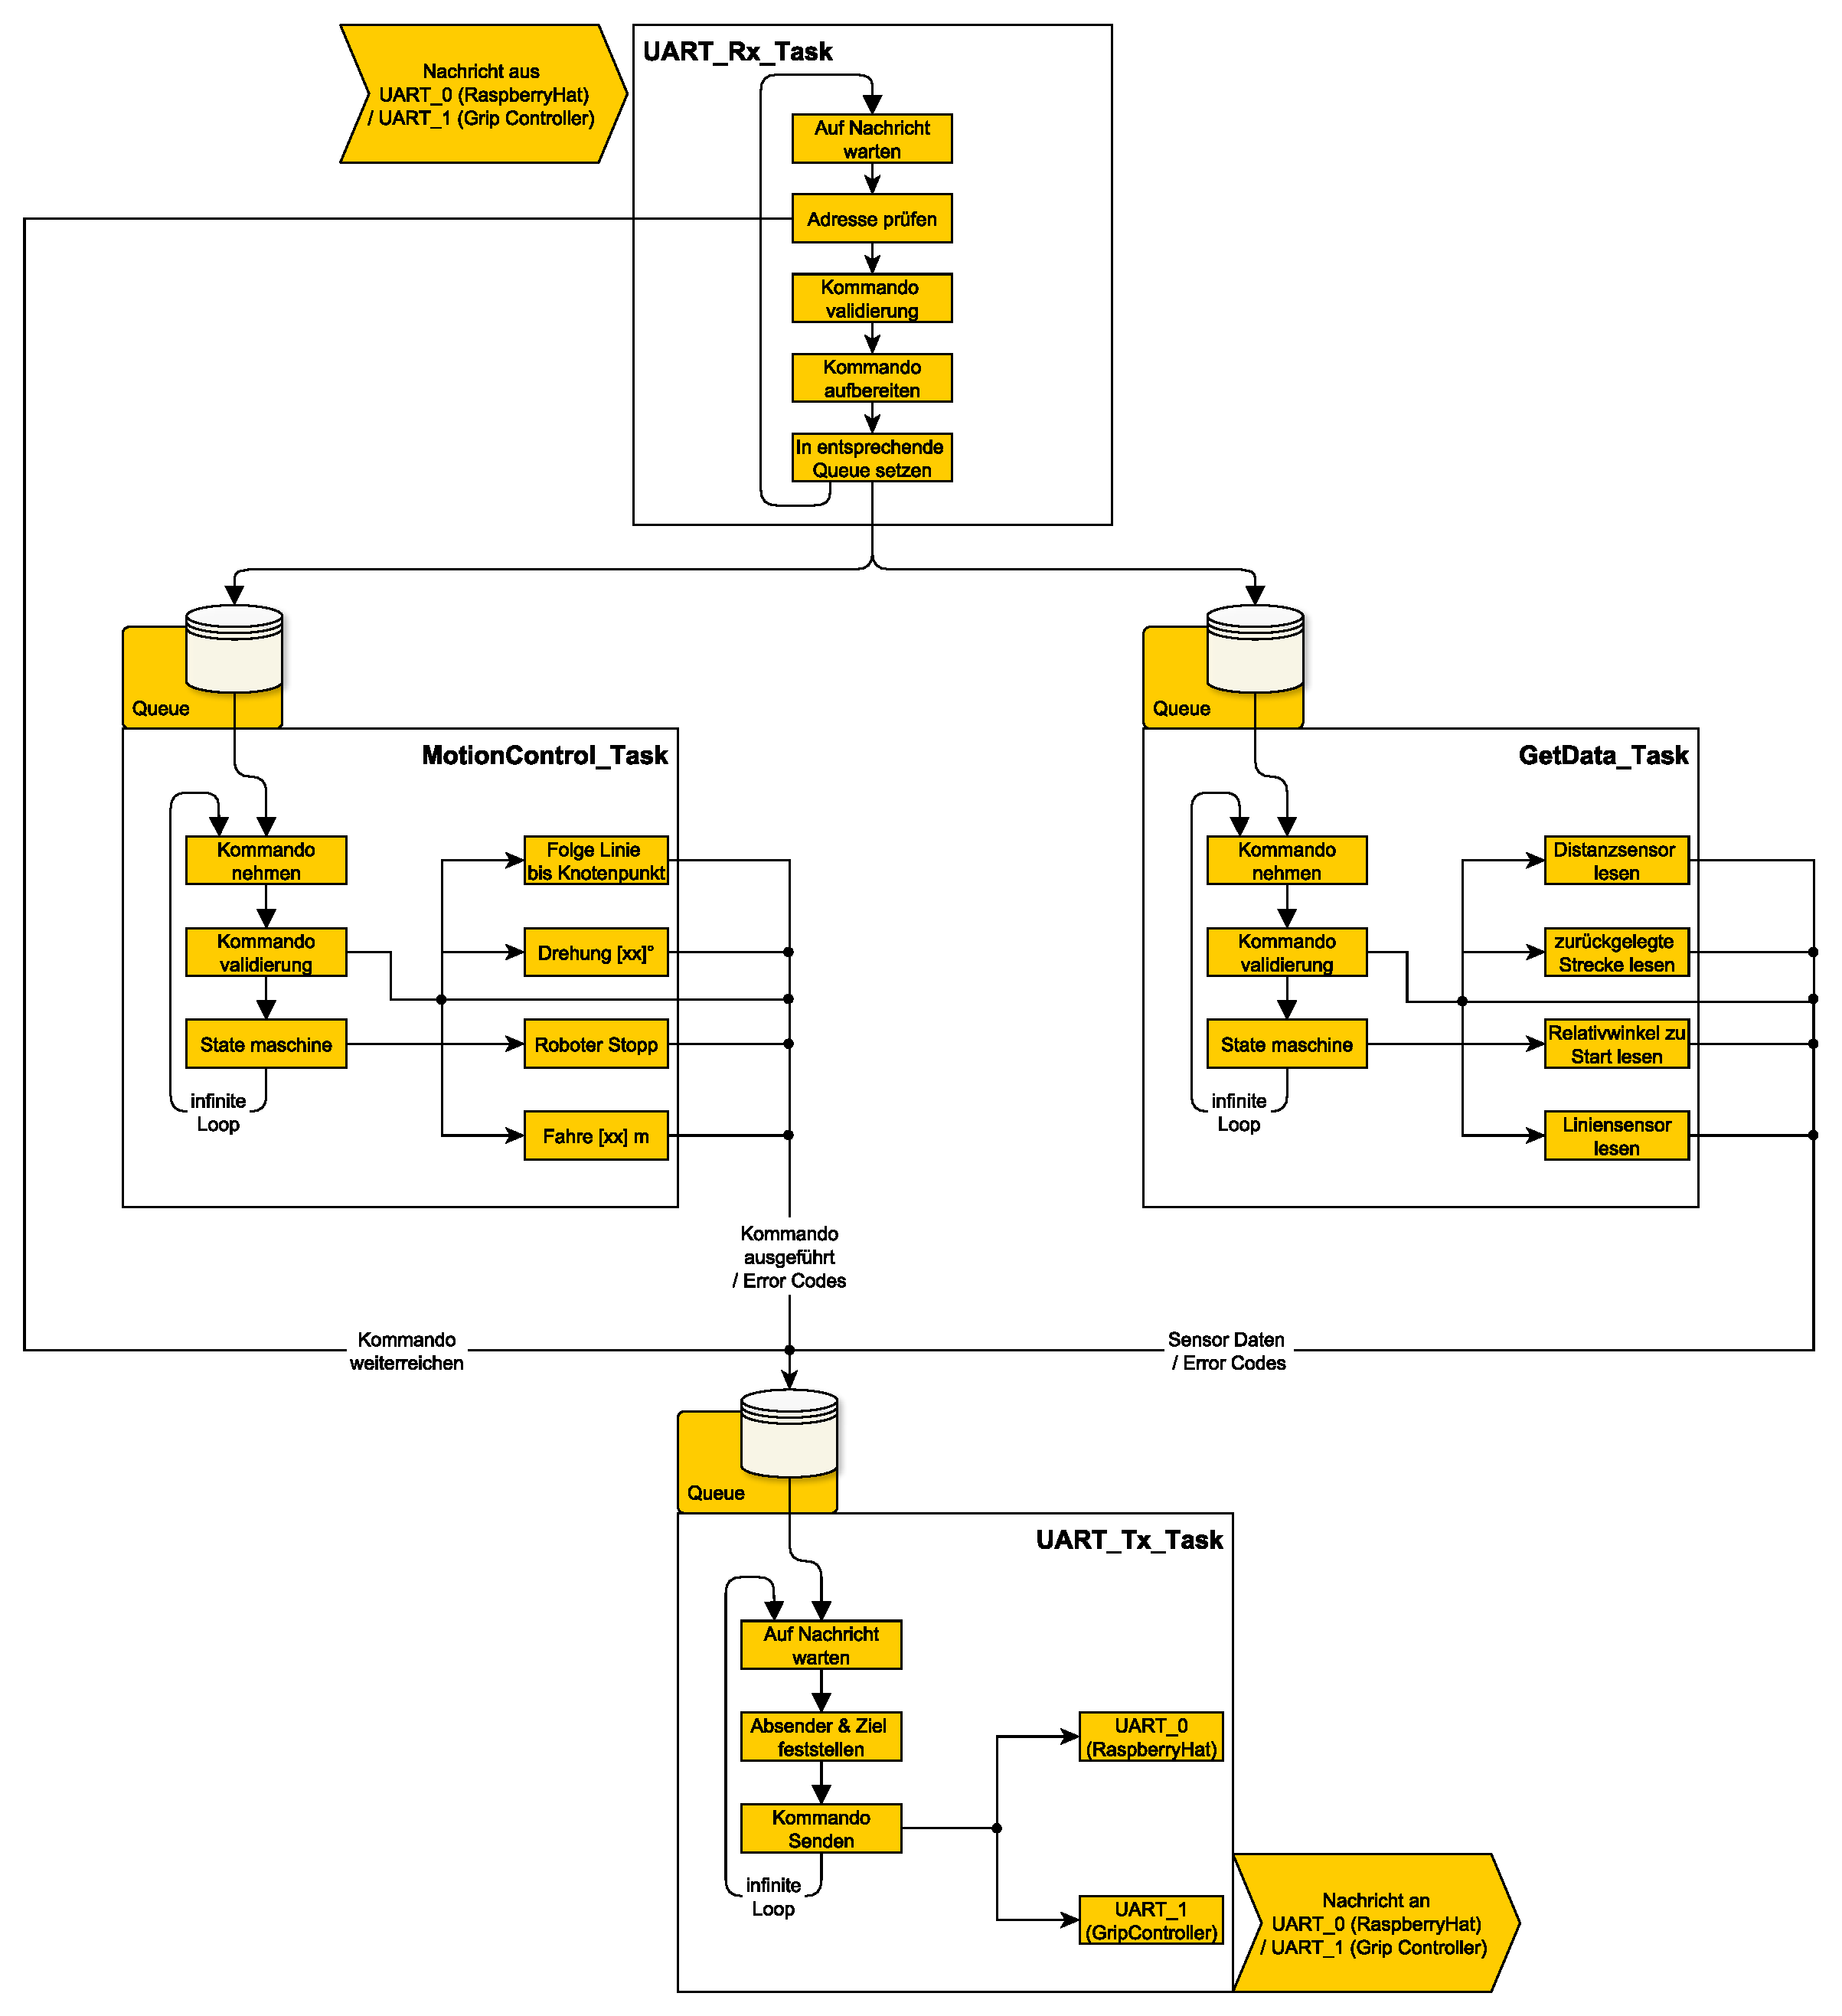
\includegraphics[width = 0.75\linewidth]{fig_Antriebe_und_Dimensionierung/Konzept_Steuerablauf.pdf}
    \caption{Steuerablauf Motion Controller}~\label{fig:MotionController_Firmware}
\end{figure}

Abbildung~\ref{fig:MotionController_Firmware} zeigt schematisch, wie die
Firmware des Motion Controllers zu implementieren ist. Es sollte eine
\textit{UART_rx}- und eine \textit{UART_tx}-Task geben, die nur auf eingehende
und ausgehende Signale warten. Dadurch wird verhindert, dass mehrere Tasks
gleichzeitig auf dieselbe UART-Schnittstelle zugreifen. Wenn der Befehl für die
Steuerung bestimmt und validiert ist, wird er in eine Queue eingereiht.
Die zugehörige Task arbeitet dann in Form einer Zustandsmaschine die
eingehenden Befehle in ihrer Queue ab. Durch diese Struktur ist die Firmware
sehr modular aufgebaut, was spätere Anpassungen oder Erweiterungen wesentlich
vereinfacht.

\begin{figure}[H]
    \centering
    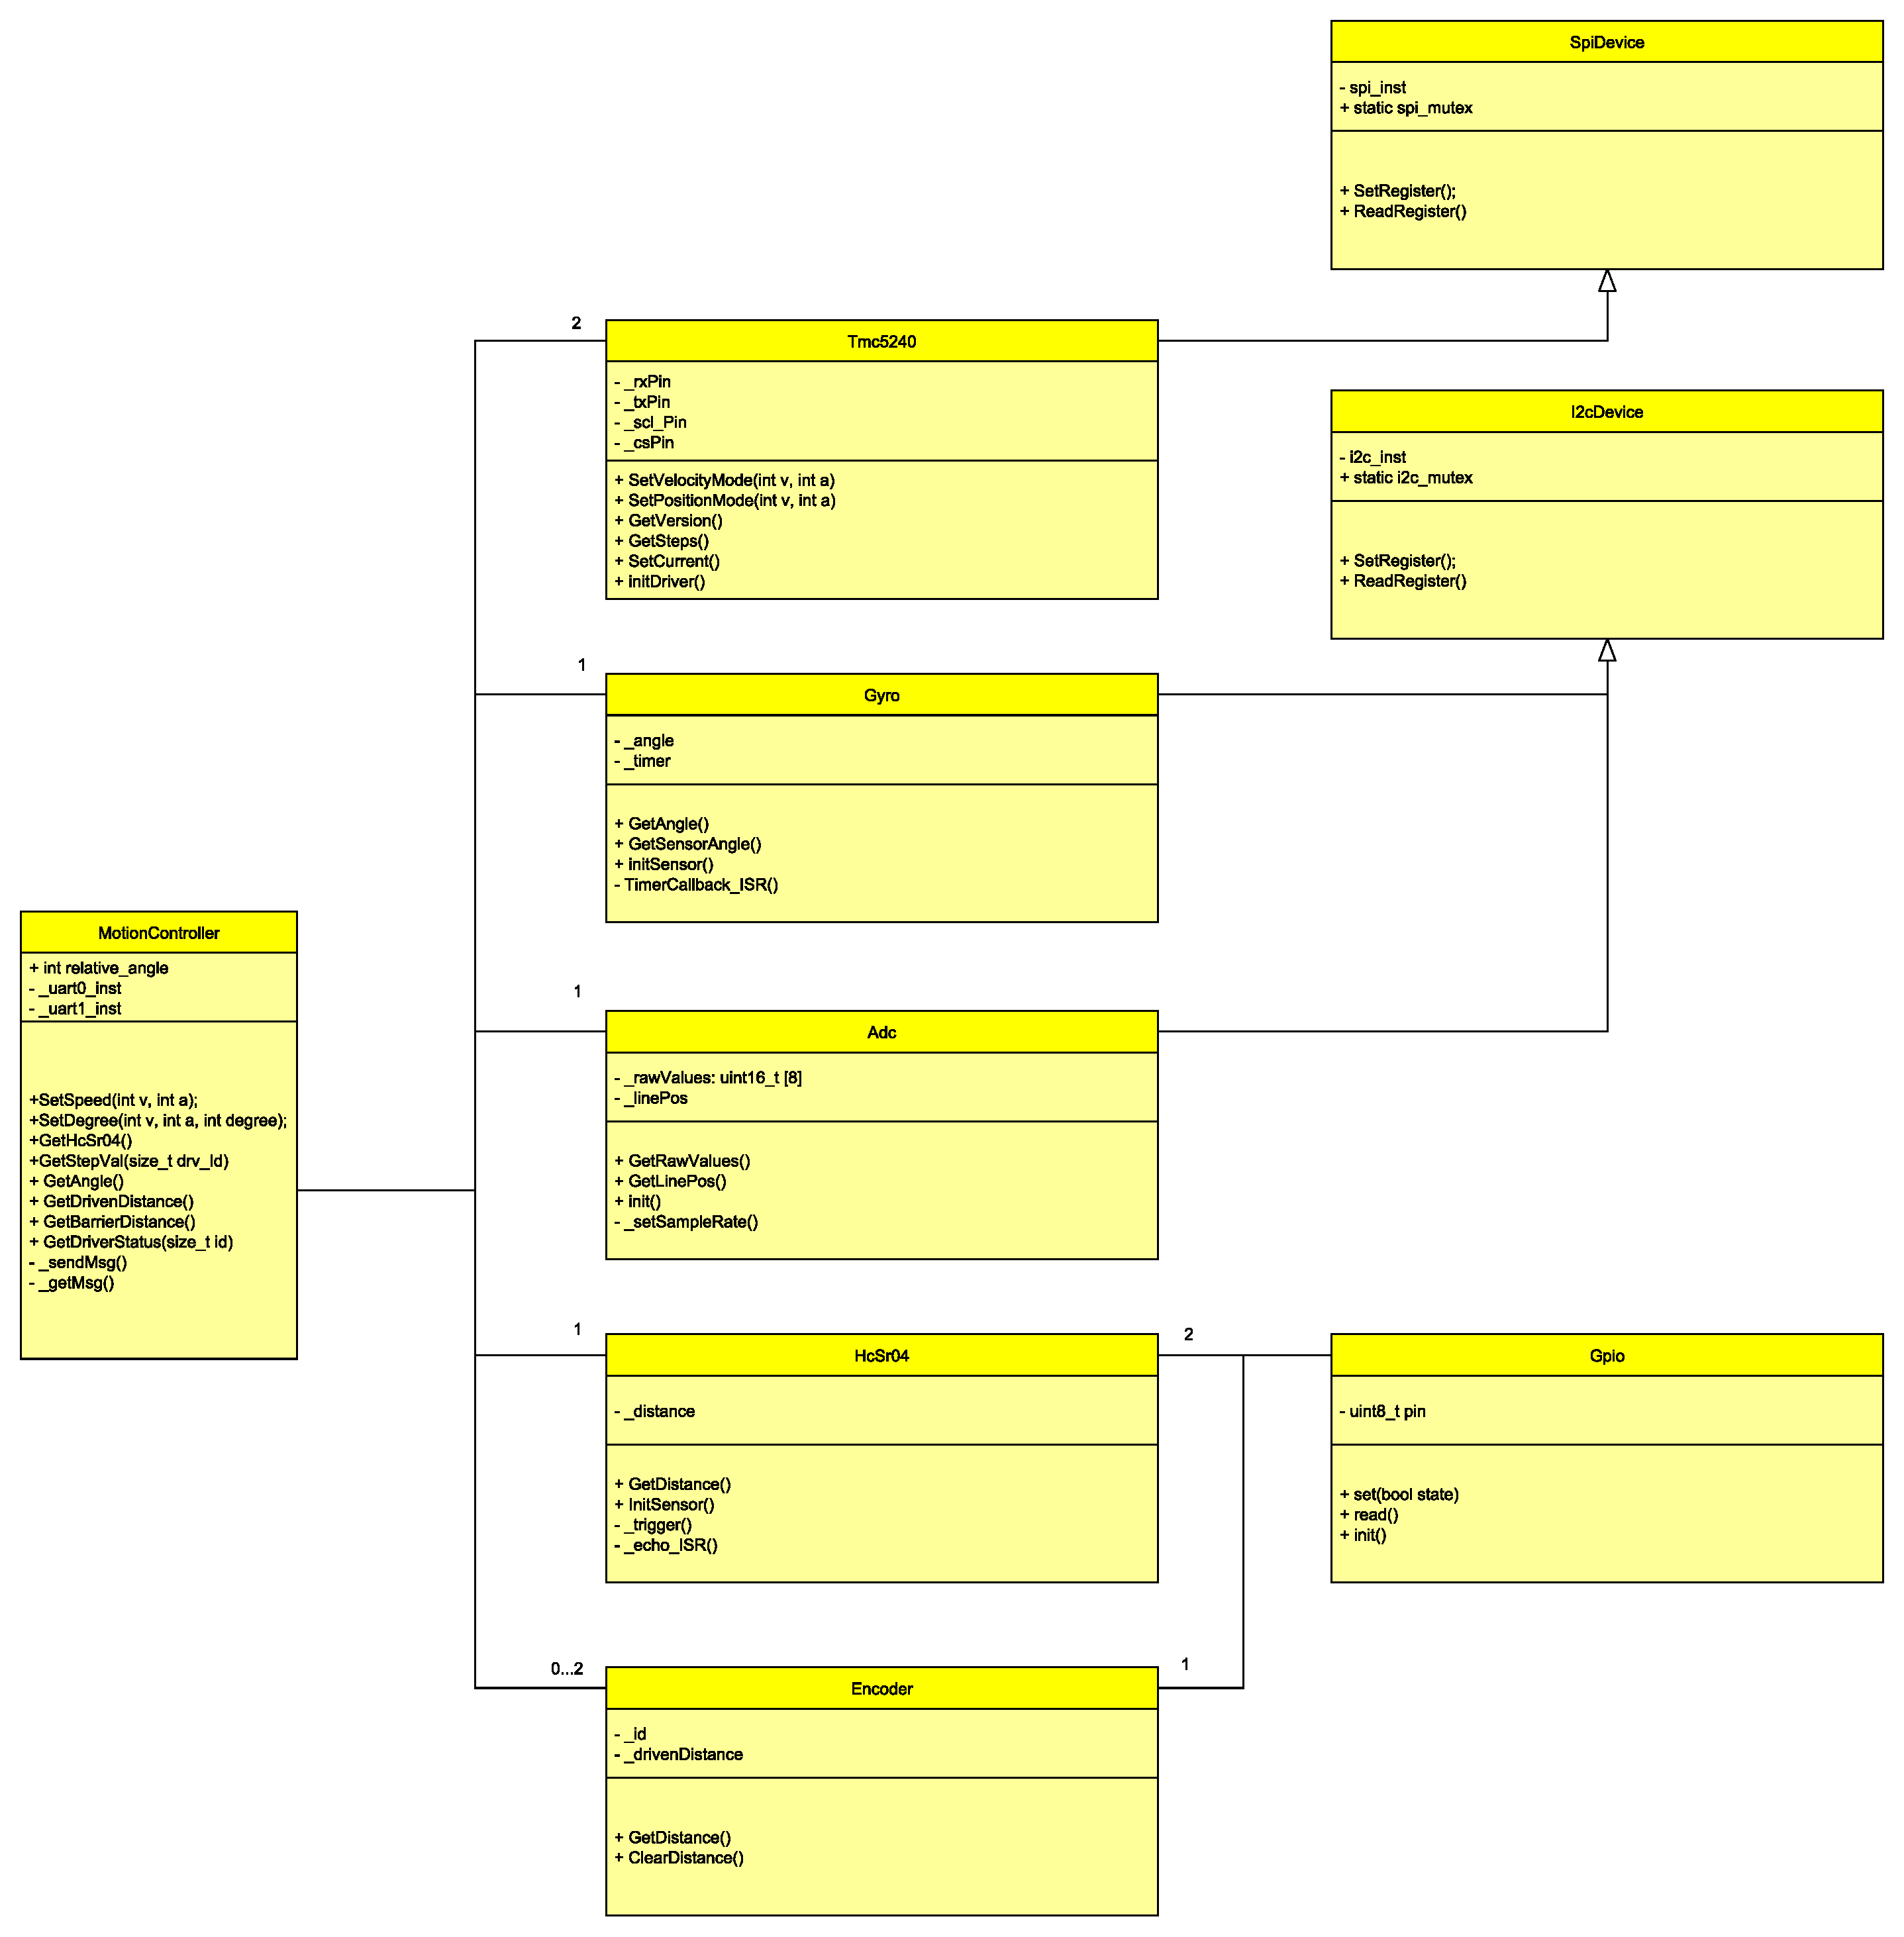
\includegraphics[width = 0.75\linewidth]{fig_Antriebe_und_Dimensionierung/Konzept_ClassDiagramm.pdf}
    \caption{Klassendiagramm Motion Controller}~\label{fig:MotionController_ClassDiagramm}
\end{figure}

In Abbildung~\ref{fig:MotionController_ClassDiagramm} ist konzeptionell
dargestellt, wie die zu erstellenden Klassen und Objekte zueinander in
Beziehung stehen.